\section{Ejecución, documentación y retroalimentación de pruebas}
%Sólo se debe registrar en el mismo formulario o documento del plan de pruebas de la etapa anterior. Se deben registrar los resultados obtenidos por la ejecución de las pruebas planificadas y las acciones correctivas realizadas, si hubieren correspondido (tengan en cuenta lo aportado por el Ing. Diego Villa).
 La retroalimentación de las pruebas para la funcionalidad del sistema elegida que se refiere a \textbf{``carga y muestra de análisis''}, se detallan al finalizar cada sprint.
 
  Los sprint donde se desarrollaron la funcionalidad elegida se detallan a continuación acompañados de una breve descripción de las actividades realizadas en cada uno de ellos.
 \begin{itemize}
 	\item \textbf{Sprint 2:} Desarrollo de la carga y muestra de mediciones, se realizaron las pruebas necesarios y se hizo la retroalimentación respectiva.
 	\item \textbf{Sprint 3:} Corrección de issues detectados por las pruebas realizadas en el sprint 2.
 	\item \textbf{Sprint 4:} Aquí se desarrolló la presentación en forma gráfica de las mediciones, se indicaron las pruebas y la retroalimentación de las mismas.
 	\item \textbf{Sprint 5:} En este sprint se desarrollo la funcionalidad de autenticación del usuario, si bien esta función no se refiere a mediciones, todo el sistema hace uso de la misma y ya sea para cargar o ver la información, el usuario debe validarse.
 	\item \textbf{Sprint 6: } Este Sprint junto al \textbf{Sprint 2} y \textbf{Sprint 7}, es el mas importante, ya que aquí se desarrolló completamente la funcionalidad que le permite cargar un análisis completo, con imágenes y mediciones,  y que luego pueda verlo de diferentes maneras, ya sea de forma gráfica, resumida o tabular.
 	\item \textbf{Sprint 7: } Aquí se desarrollo la funcionalidad que le permite al usuario cargar un archivo y/o imagen, YesDoc guarda estos documentos en una cuenta de dropbox solo accedida por el usuario autorizado.
 \end{itemize}
 

 Para facilitar la lectura de la ejecución, documentación y retroalimentación de pruebas, a continuación, se acerca un ejemplo de cada tipo de prueba realizada para la funcionalidad seleccionada y al finalizar se añade  una síntesis del resultado del total de las pruebas realizadas.
  \subsection{Ejecución y documentación de pruebas}
  
  \subsubsection{Pruebas de unidad}
  
  \begin{lstlisting}[language=Python ]
  class MeasurementResourceTestCase(unittest.TestCase):
  
  def setUp(self):
  self.app = app
  self.app_context = self.app.app_context()
  self.app_context.push()
  db.create_all()
  
  def tearDown(self):
  db.session.remove()
  db.drop_all()
  self.app_context.pop()
  
  def test_measurement(self):
  g1 = Gender(name='femenino', description='Sexo femenino.')
  p1 = Profile(last_name='Correa', first_name='Laura', birthday='1998-08-20', gender_id='1')
  p2 = Profile(last_name='Correa', first_name='Ana', birthday='1998-04-10', gender_id='1')
  ms1 = MeasurementSource(name='Manual', description='Ingreso manual de la medida.')
  mu1 = MeasurementUnit(name='Kilogramo', symbol='kg', suffix='True')
  mt1 = MeasurementType(name='Peso', description='Medida de peso de una persona')
  u1 = User(username='lcorrea', password='l5ur5', email='lcorrea@yesdoc.com', profile_id='1')
  u2 = User(username='acorrea', password='5n5', email='acorrea@yesdoc.com', profile_id='2')
  a1 = Analysis(datetime='2015-10-15 22:58:11.963369', description='Primer toma de medidas de peso',
  profile_id='1')
  m1 = Measurement(datetime='2015-10-15 23:05:52.393670', value='74', analysis_id='1', profile_id='1',
  source_id='1', type_id='1', unit_id=1)
  mt1.measurement_units.append(mu1)
  db.session.add_all([g1, p1, p2, ms1, mu1, mt1, u1, u2, a1, m1])
  db.session.commit()
  
  # Preparacion del token
  token = u1.generate_auth_token(360)
  token = base64.b64encode(token + ':')
  token_a = 'sdalnlkkkl349aslnf03rnl'
  
  # test resource: MeasurementList, method: POST, response_code: 201, con autorizacion
  with self.app.test_request_context(
  '/measurements',
  method='POST',
  data=json.dumps({'datetime': '2015-10-22 17:34:02.175126', 'value': 70, 'analysis_id': 1,
  'profile_id': 1, 'measurement_source_id': 1, 'measurement_type_id': 1,
  'measurement_unit_id': 1}),
  headers={'Content-Type': 'application/json', 'Authorization': 'Basic ' + token}):
  res = self.app.full_dispatch_request()
  data = json.loads(res.data)
  self.assertTrue(data['resource']['id'] == 2)
  self.assertTrue(data['resource']['datetime'] == '2015-10-22T17:34:02.175126')
  self.assertTrue(data['resource']['value'] == 70)
  self.assertTrue(res.status_code == 201)
  
  # test resource: MeasurementList, method: POST, response_code: 401, sin autorizacion, token invalido
  with self.app.test_request_context(
  '/measurements',
  method='POST',
  data=json.dumps({'datetime': '2015-10-22 17:34:02.175126', 'value': 68, 'analysis_id': 1,
  'profile_id': 1, 'measurement_source_id': 1, 'measurement_type_id': 1,
  'measurement_unit_id': 1}),
  headers={'Content-Type': 'application/json', 'Authorization': 'Basic ' + token_a}):
  res = self.app.full_dispatch_request()
  print res
  self.assertTrue(res.status_code == 401)
  
  # test resource: MeasurementList, method: GET, response_code: 200
  with self.app.test_request_context(
  '/measurements',
  method='GET',
  data=json.dumps({}),
  headers={'Content-Type': 'application/json'}):
  res = self.app.full_dispatch_request()
  data = json.loads(res.data)
  self.assertTrue(len(data['resource']) == 2)
  self.assertTrue(res.status_code == 200)
  
  # test resource: MeasurementView, method: GET, response_code: 200
  with self.app.test_request_context(
  '/measurements/1',
  method='GET',
  data=json.dumps({}),
  headers={'Content-Type': 'application/json'}):
  res = self.app.full_dispatch_request()
  data = json.loads(res.data)
  self.assertTrue(len(data) == 1)
  self.assertTrue(data['resource']['value'] == 74)
  self.assertTrue(res.status_code == 200)
  
  # test resource: MeasurementView, method: GET, response_code: 404
  with self.app.test_request_context(
  '/measurements/3',
  method='GET',
  data=json.dumps({}),
  headers={'Content-Type': 'application/json'}):
  res = self.app.full_dispatch_request()
  self.assertTrue(res.status_code == 404)
  \end{lstlisting}
  
  \subsubsection{Pruebas de carga}
  Se va a simular el acceso a la página hosteada en Heroku, de un lote de usuarios. Además en la gráfica \textbf{[Figura \ref{prueba_carga_50_us}]}se puede ver los tiempos de respuesta al ir incrementando la cantidad de usuarios.
  
  \begin{center}
  	\begin{tabular}{|c|c|}
  		\hline Cantidad de Usuario  &  Tiempo de espera\\ 
  		\hline 20 usuarios &  155 ms \\ 
  		\hline 30 usuarios  & 115 ms \\ 
  		\hline 40 usuarios  & 100 ms \\ 
  		\hline 50 usuarios  & 130 ms \\ 	
  		\hline 
  	\end{tabular} 
  \end{center}
  
  \begin{figure}[h]
  	\centering
  	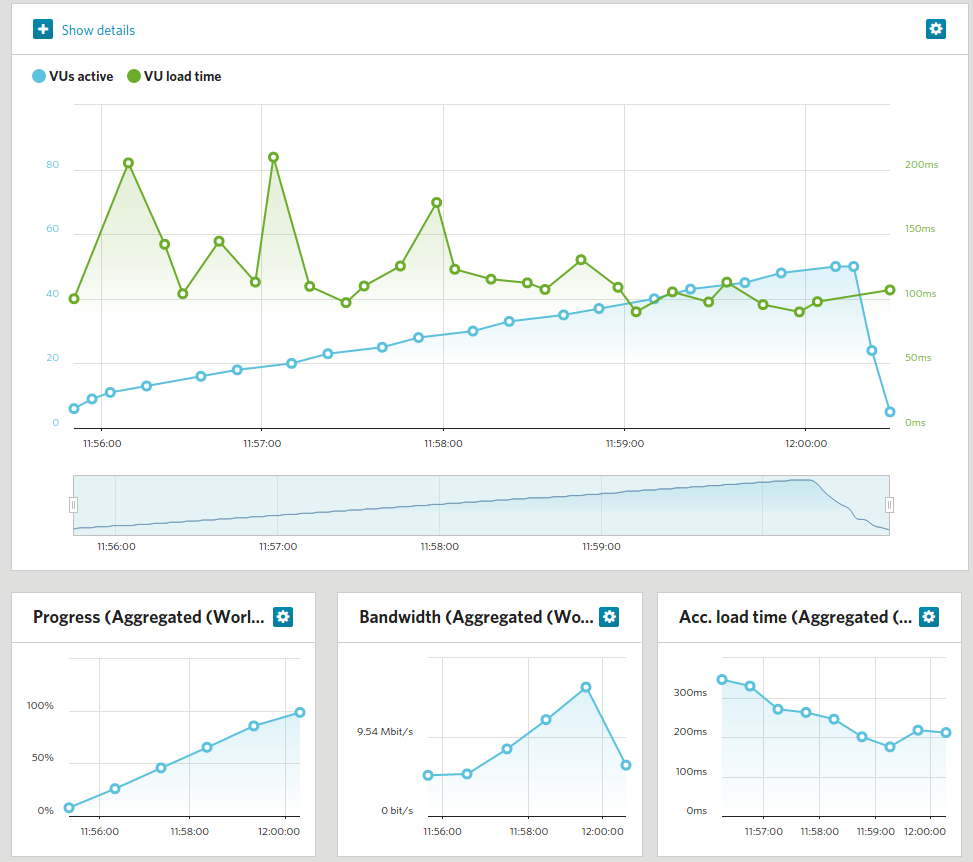
\includegraphics[width=0.5\textwidth]{img/prueba_carga_50_us}
  	\caption{Prueba de carga simulando 50 usuarios}
  	\label{prueba_carga_50_us}
  \end{figure}
  
  Se puede observar que en promedio el tiempo de carga se mantiene regular aunque vaya en aumento la cantidad de usuarios.
  
  \subsubsection{Pruebas de performance}
  Google developers mide de 0 a 100 la velocidad de carga del sitio e indica, por orden de prioridad, qué mejorar, aportando información al respecto.
  en nuestro caso nos recomienda disminuir el tamaño de las imágenes \textbf{[Figura \ref{prueba_velocidad_1}]}
  
  \newpage
  
  \begin{figure}[h]
  	\centering
  	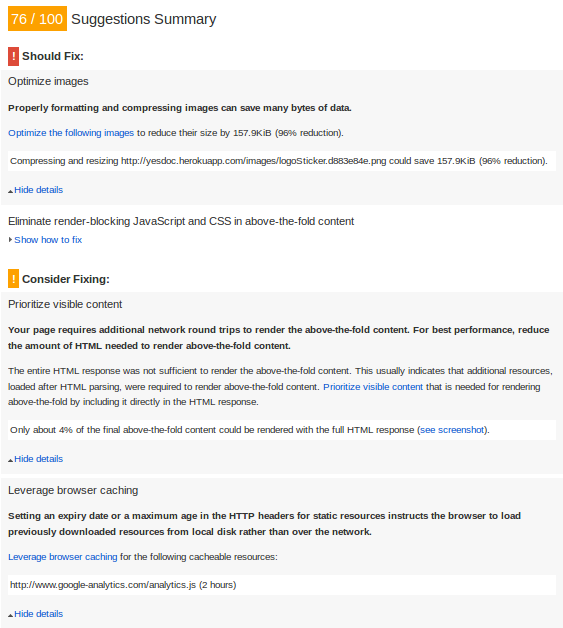
\includegraphics[width=0.5\textwidth]{img/prueba_velocidad_1}
  	\caption{Pruebas de velocidad en desktop}
  	\label{prueba_velocidad_1}
  \end{figure}
  
  \begin{figure}[h]
  	\centering
  	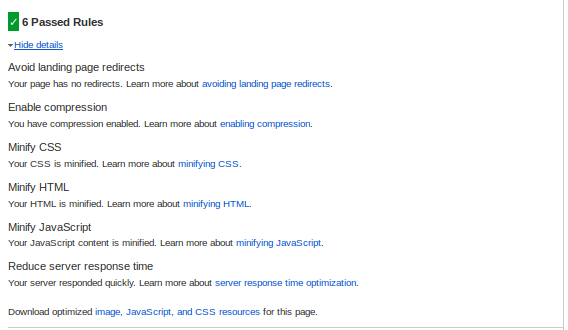
\includegraphics[width=0.5\textwidth]{img/prueba_velocidad_2}
  	\caption{Pruebas de velocidad pasadas}
  	\label{prueba_velocidad_2}
  \end{figure}
  \subsubsection{Pruebas de seguridad por niveles de usuario}
  
  \begin{longtable}{|p{1.0cm}|p{4cm}|p{4cm}|p{4cm}| }
  	
  	\hline
  	\rowcolor[gray]{0.9} 
  	\multicolumn{1}{|c}{Id test seguridad} & \multicolumn{1}{|c|}{Contexto} & \multicolumn{1}{|c|}{Evento} & \multicolumn{1}{|c|}{Resultado esperado} \\
  	\hline
  	ST-1 & Si el token utilizado en el header Authorization de la solicitud no corresponde a un usuario del sistema  & al solicitar el servicio put del recurso AnalysisView & El sistema retorna una respuesta con código de estado HTTP 401, UNAUTHORIZED\\
  	\hline
  	ST-2 & Si el token utilizado en el header Authorization de la solicitud corresponde a un usuario del sistema pero no al usuario al que pertenece el analysis & al solicitar el servicio put del recurso AnalysisView & El sistema retorna una respuesta con código de estado HTTP 403, FORBIDDEN\\
  	\hline
  	ST-3 & Si el token utilizado en el header Authorization de la solicitud corresponde a un usuario del sistema, el análisis con el identificador existe y el token pertenece al usuario al que pertenece el análisis & al solicitar el servicio put del recurso AnalysisView & El sistema retorna en el cuerpo de la respuesta los datos del análisis y el código de estado HTTP 200, UPDATED\\
  	\hline
  	ST-4 & Si el token utilizado en el header Authorization de la solicitud corresponde a un usuario del sistema, el análisis con el identificador existe y el token pertenece al usuario al que pertenece el análisis & al solicitar el servicio delete del recurso AnalysisView & El sistema retorna la respuesta con código de estado HTTP 204, DELETED\\
  	\hline
  	
  \end{longtable}
  
  \begin{center}
  	\begin{longtable}{|m{4cm}|m{4cm}|m{3cm}|m{2cm}|}
  		\hline \hline \rowcolor[gray]{0.9}
  		\multicolumn{4}{|c|}{\textbf{Procedimiento de pruebas}} \\
  		\hline 
  		
  		\multicolumn{4}{|c|}{\textbf{Descripción de escenario}: Debe hacer las pruebas un usuario no autenticado.} \\
  		\hline 
  		
  		\rowcolor[gray]{0.9}
  		\multicolumn{1}{|c|}{\textbf{Actor}} &
  		\multicolumn{1}{c|}{\textbf{Sistema}} &
  		\textbf{Resultado esperado}&
  		\textbf{Resultado obtenido} \\
  		\hline
  		El usuario ingresa a la URL \url{https:// yesdoc.herokuapp.com/#/profileMeasurements}.
  		&
  		El sistema consulta a la API si el token se encuentra activo, la API devuelve un error 401, \textbf{[Figura \ref{no_autorizado_profile_measurement}]}.
  		&
  		Se redirige al usuario al formulario de login.
  		&
  		Correcto.
  		\\ 
  		\hline
  		El usuario ingresa a la URL \url{https:// yesdoc.herokuapp.com/#/profileInformation}.
  		&
  		El sistema consulta a la API si el token se encuentra activo, la API devuelve un error 401, \textbf{[Figura \ref{no_autorizado_profile_measurement}]}.
  		&
  		Se redirige al usuario al formulario de login.
  		&
  		Correcto.
  		\\ 
  		\hline
  		El usuario ingresa a la URL \url{https:// yesdoc.herokuapp.com/#/home}.
  		&
  		El sistema consulta a la API si el token se encuentra activo, la API devuelve un error 401, \textbf{[Figura \ref{no_autorizado_profile_measurement}]}.
  		&
  		Se redirige al usuario al formulario de login.
  		&
  		Correcto.
  		\\ 
  		\hline
  		
  	\end{longtable}
  \end{center}
  \subsubsection{Pruebas de integración}
  
  {\scriptsize
  \begin{longtable}{|p{4cm}|p{4cm}|p{4cm}|p{3cm}|}
  	\hline
  	Actor  & Sistema& Resultado Esperado & Resultado obtenido \\ \hline
  	
  	El usuario intenta ingresar al sistema & El sistema valida que el usuario con la contraseña ingresada exista 
  	& Se muestra un cartel de aviso de \textbf{usuario o contraseña invalido} 
  	& Ok, aunque el cartel podría ser mas vistoso 
  	\\ \hline
  	
  	
  	
  	El usuario selecciona \textbf{nuevo perfil}, para
  	crear una cuenta en YesDoc 
  	& El sistema direcciona a la vista de creación de perfil
  	& Muestra formulario de creación de perfil.
  	&
  	\\ \hline
  	
  	
  	
  	El usuario completa todos los campos y presiona save.
  	Ingresa:
  	\begin{itemize}
  		\item \textbf{Nombre de usuario:} Franco
  		\item \textbf{Apellido:} Canizo
  		\item \textbf{Fecha de nacimiento: }2015-10-90
  		\item \textbf{Género: }Masculino
  		\item \textbf{Email: }franco@franco
  		\item \textbf{pass:}Franco
  		
  	\end{itemize}
  	& El sistema anula el botón \textbf{guardar }hasta tanto el usuario cargue todos los campos. una vez cargado todos los campos,al presionar save, redirecciona al menu
  	de logueo de usuario.
  	& El sistema informa que ha sido generado su usuario y lo direcciona al formulario de login.
  	& Ok, pero muestra ciertos mensajes de error al enviar el formulario \textbf{[Issue \#50]}
  	\\ \hline
  	
  	
  	
  	El usuario ingresa 
  	\textit{\begin{itemize}
  			\item \textbf{Nombre de usuario:}Franco
  			\item \textbf{Password: }Franco
  		\end{itemize} }
  		&	El sistema valida usuario y contraseña,genera el token, direcciona a myProfileInformation y consulta a la API por la información personal \textbf{Figura \ref{5-login}}
  		& Se muestra la vista de perfil del usuario indicando sus datos personales
  		\begin{itemize}
  			\item \textbf{Nombre de usuario:} Franco 
  			\item \textbf{Apellido: }Canizo 
  			\item \textbf{Fecha de nacimiento: }2015-10-90 
  			\item \textbf{Género: }Masculino
  		\end{itemize}
  		& Todo Ok, pero podrían aumentarse los colores y quitar espacios en blanco
  		\\ \hline
  		
  		
  		Presiona el boton \textit{\textbf{``Editar Perfil'' }}
  		& El sistema carga la vista \textbf{``profileinformation-edit.html''}, carga la vista correspondiente , valida que el usuario se encuentre logueado pasándole el token que se encuentra almacenado en las cookies. Solicita ala API los datos del perfil y del genero
  		para rellenar el formulario.
  		& Se muestra el formulario con los datos del perfil a editar.
  		& No carga los datos del usuario \textbf{[Issue \#47]}
  		\\ \hline
  		
  		
  		
  		Cambia
  		\textit{
  			\begin{enumerate}
  				\item \textbf{Nombre de usuario :} Franco Nicolás
  			\end{enumerate}}
  			&
  			& Muestra el cambio
  			& Ok
  			\\ \hline
  			
  			
  			Guarda los datos presionando en \textit{\textbf{``guardar''}} 
  			& El sistema se conecta con la API y guarda los datos a través del método PUT. Redirecciona al perfil de usuario y muestra los datos cambiados
  			&
  			Se muestra el perfil con los.
  			\textit{
  				\begin{itemize}
  					\item \textbf{Nombre de usuario:} Franco Nicolas
  					\item \textbf{Apellido:} Canizo
  					\item \textbf{Fecha de Nacimiento: }2015-10-90
  					\item \textbf{Género:} Masculino
  					\item \textbf{Email: }franco@franco
  				\end{itemize}
  			}
  			& Guarda bien, pero al enviar el formulario muestra errores de validación \textbf{[Issue \#50]}
  			\\ \hline
  			
  			
  			El usuario presiona en \textbf{``Resumen'' } para ir a la sección donde se muestra una lista de cada medición con su último valor cargado.
  			
  			& El sistema cambia la url por \textit{\textbf{``\#pro-fileMeasurements''}}, carga la vista correspondiente, valida que el usuario se encuentre logueado pasándole el token que se encuentra almacenado en las cookies y solicita al recurso de la API \textit{\textbf{``my/measurements/latest'' }}las últimas mediciones de cada tipo del usurario. \textbf{Figura \ref{5-perfil}}
  			
  			& Se muestra una pantalla con dos botones uno para la carga de medición
  			\textit{\textbf{``Nueva Medición'' }}y otro para la carga de análisis \textit{\textbf{``Nuevo Análisis''}}. No se muestra más datos porque es un usuario nuevo sin información.\textbf{Figura \ref{5-perfil_mediciones}}
  			& OK
  			\\ \hline
  			
  			
  			
  			Selecciona en \textbf{``Nueva análisis'' }
  			& El sistema direcciona a la url \textit{\textbf{"analy-sis/new"}}, carga la vista correspondiente, valida que el usuario se encuentre logueado pasándole el token que se encuentra almacenado en las cookies.
  			
  			& Se muestra el formulario de carga de análisis \textbf{[Figura \ref{5-crear_analisis} ]}
  			& ok
  			\\ \hline
  			
  			
  			
  			El usuario carga
  			
  			\begin{itemize}
  				\item \textbf{Fecha :}2015-09-30 16:10:59
  				\item \textbf{Descripción: }revisión general
  				\item Presionar en .\textbf{``Adjuntos''}
  				
  			\end{itemize}
  			
  			&
  			& El sistema muestra una ventana donde se puede cargar las imágenes con la medición y fecha.\textbf{ [Figura  \ref{5-cargar_img}]}
  			&ok
  			
  			\\ \hline
  			
  			
  			
  			Selecciona una imagen "jpg.o "png", de-ja la fecha igual. 
  			&
  			& Se muestra una imagen previa de la imagen. Se muestra la fecha En descripción se muestra el nombre de la imagen
  			& ok
  			\\ \hline
  			
  			
  			
  			Presiona \textbf{\textit{``guardar''}}
  			&
  			& Muestra
  			\begin{itemize}
  				\item Nombre de la descripción de la imagen.
  				\item Iconos de visualizar,
  				\item \textbf{Iconos de editar}
  				\item \textbf{Iconos de borrar.}
  			\end{itemize}
  			& ok
  			\\ \hline
  			
  			
  			
  			
  			
  			Seleccionar \textit{\textbf{``cargar Medición'' }}
  			& El sistema se conecta con la API para solicitar tipo y fuentes de mediciones
  			& El sistema muestra una ventana donde  se puede cargar las mediciones con los siguientes datos:
  			\textbf{\begin{itemize}
  					\item ``Tipo'',
  					\item ``Valor''
  					\item ``Unidad''
  					\item ``Fuente''
  					\item ``Fecha''
  				\end{itemize}}
  				\textbf{[Figura \ref{5-cargar_medicion}]}
  				& ok
  				\\ \hline
  				
  				
  				
  				
  				Selecciona tipo:\textit{\textbf{ "peso"} }
  				& El sistema se conecta con la API para
  				solicitar unidades relacionadas al tipo de medición peso con \textbf{id:``1'' }. \textbf{[Figura \ref{5-crear_medicion}]}
  				& Muestra las posibles unidades correspondientes al tipo peso
  				& ok
  				\\ \hline
  				
  				
  				
  				Ingresa
  				\begin{itemize}
  					\item \textbf{Tipo:} ``Peso''
  					\item \textbf{valor: }``65''
  					\item \textbf{Unidad:} ``kilogramo''
  					\item \textbf{Fuente: }``manual''
  					\item \textbf{Fecha: }``2015:-09-30 16:10:59''
  					\item \textbf{ Guardar}
  				\end{itemize}
  				&
  				& Mantiene la misma venta abierta y muestra un mensaje de aviso de que la
  				medición fue cargada con éxito.\textit{ \textbf{"Bien hecho se cargo una medición''}}
  				& ok, si bien es útil que mantenga los datos para facilitar la nueva carga, sería conveniente acentuar el aviso de que la medición ya se cargo.
  				\\ \hline
  				
  				
  				
  				
  				
  				Modificado el valor ingresado con anterioridad
  				
  				\begin{itemize}
  					\item \textbf{Tipo:} ``Peso''
  					\item \textbf{valor: }``75''
  					\item \textbf{Unidad:} ``kilogramo".
  					\item \textbf{Fuente: }``manual"
  					\item \textbf{Fecha: }2015:-10-10 16:10:59
  					\item \textbf{ Guardar}
  				\end{itemize}
  				&
  				& Mantiene la misma venta abierta y muestra un mensaje de aviso de que la
  				medición fue cargada con éxito.\textbf{``Bien hecho se cargo una medición''}
  				& ok
  				\\ \hline
  				
  				
  				
  				
  				Selecciona
  				
  				
  				
  				\begin{itemize}
  					\item \textbf{Tipo:} ``altura'', modifica el valor ingresado con anterioridad
  					por
  					\item \textbf{valor: }``170''
  					\item \textbf{Unidad:} ``centímetro".
  					\item \textbf{Fuente: }``manual"
  					\item \textbf{Fecha: }2015:-10-23 16:10:59
  					\item \textbf{ Guardar}
  				\end{itemize}
  				&
  				&
  				Mantiene la misma venta abierta y muestra un mensaje de aviso de que
  				la medición fue cargada con éxito.\textit{\textbf{ ``Bien hecho se cargo una medición''}}
  				& ok
  				\\ \hline
  				
  				
  				
  				
  				Se selecciona el botón \textbf{"guardar"}
  				& El sistema consulta el perfil a la API para extraer el id el cual se usara para crear un análisis. Envía por POST a la API el análisis y realiza tres llamados mas a la API uno por cada medición cargada.
  				Mantiene la misma venta abierta y muestra un mensaje de aviso de que
  				la medición fue cargada con éxito. Almacena en la API el path y el storage\_location de la imagen.Luego direcciona la página a la url
  				\textit{\textbf{\#/profileMeasurements}}, valida que el token se encuentre activo, si no hay
  				errores solicita a la API las ultimas mediciones y muestra las mediciones
  				
  				& En la vista de perfil de mediciones,Lista las últimas mediciones cargadas,
  				mostrando el peso cargado mas recientemente
  				
  				\begin{itemize}
  					\item Peso: 65 Kg Fecha 2015-10-2314:42:56 Manual
  					\item Altura: 170 cm 2015-10-2314:42:56 Manual
  					
  				\end{itemize}
  				& ok, habría que explicar que para ver todos sus pesos debería dirigirse a histórico
  				
  				\\ \hline
  				
  				
  				
  				
  				
  				
  				Selecciona el icono de edición ubicado al lado de la medición \textit{Peso 65Kg}
  				& El sistema redirecciona \textbf{\#/measure-ments/103/edit}, verifica con la API que el token se encuentre activo, a partir del\textbf{ id} de la medición seleccionada para editar trae de la API el \textbf{tipo de medición, el valor, la unidad, la fuente y la fecha.}
  				
  				& Se muestra un formulario con los datos de la medición precargadas
  				\begin{itemize}
  					\item \textbf{Tipo:}Peso 
  					\item \textbf{Valor: }65 
  					\item \textbf{Unidad:} kilogramo
  					\item \textbf{Fuente:}Manual 
  					\item \textbf{Fecha:}2015-10-23 -14:42:56
  				\end{itemize}
  				&  ok
  				\\ \hline
  				
  				
  				
  				
  				
  				Cambia la \textit{\textbf{fecha y la hora} por 2015-5-13- 4:42:56 }y guarda los cambios.
  				& El sistema guarda la medición, redirecciona\textbf{ \#/profileMeasurements }valida el token, y solicita las últimas mediciones a la API
  				
  				& Muestra la interfaz con las últimas mediciones 
  				\begin{itemize}
  					\item Peso: 75 Kg 2015-10-23 14:42:56 Manual 
  					\item Altura: 170 cm 2015-10-23 14:42:56 Manual
  				\end{itemize}
  				& ok
  				\\ \hline
  				
  				
  				
  				
  				
  				El usuario selecciona en \textit{\textbf{nueva medición}}
  				& El sistema redirecciona a \textbf{\#/measure-ments/new} valida contra la API que el Token se encuentra activo, luego trae los tipos de mediciones
  				
  				& Muestra el formulario para cargar una medición con los siguientes valores 
  				\textbf{\begin{itemize}
  						\item Tipo: 
  						\item Valor:
  						\item  Unidad: 
  						\item Fuente: 
  						\item Fecha:
  					\end{itemize}}
  					& ok
  					\\ \hline
  					
  					
  					
  					
  					
  					
  					El usuario selecciona en \textbf{``nueva medición''} 
  					\begin{itemize}
  						\item \textbf{Tipo:}Peso
  						\item \textbf{ Valor: }70
  						\item\textbf{ Unidad:}-kilogramo
  						\item \textbf{Fuente:}Manual
  						\item \textbf{ Fecha:}2015-19-23 -14:42:56 
  						\item \textbf{Guardar}
  					\end{itemize}
  					
  					& El sistema redirecciona a \textbf{\#/profile-Measurementsvalida }contra la API que el Token se encuentra activo y luego trae las últimas mediciones
  					
  					& Muestra la lista de últimas mediciones
  					\textbf{\begin{itemize}
  							\item Peso: 75 Kg 2015-10-23 14:42:56 Manual
  							\item Altura: 170 cm 2015-10-23 14:42:56 Ma-nual
  						\end{itemize}}
  						& ok
  						\\ \hline
  						
  						
  						
  						
  						Presionar en sección \textbf{``histórico''}
  						& El sistema redirecciona a\textbf{ \#/home }y se carga la vista correspondiente a  \textbf{  weight,} se verifica que el token este activo, se traen todas las medidas de tipo peso
  						& Se muestra una botonera con los tipos de mediciones , una gráfica y una tabla con las 3 medidas de tipo \textbf{Peso}
  						& ok, la botonera debería ser horizontal
  						\\ \hline
  						
  						
  						
  						
  						Presionar en sección \textbf{Altura }
  						& El sistema carga la vista correspondiente a height, se verifica que el token este activo, se traen todas las medidas de tipo peso
  						& Se muestra una botonera con los tipos de mediciones , una gráfica y una tabla con una medida \textbf{170 centímetros} de la altura.
  						& ok
  						\\ \hline
  						
  						
  						
  						
  						
  						Presionar en sección \textit{\textbf{Análisis }} 
  						& El sistema carga la vista correspondiente a análisis, se verifica que el token este activo, se traen los análisis de la API
  						& Se muestra el análisis cargado con anterioridad mostrando la imagen, la descripción y la fecha seleccionada por el usuario.
  						& ok
  						\\ \hline
  						
  						
  						
  						
  						
  						
  						Selecciona el \textit{\textbf{Análisis}}
  						& El sistema carga la vista correspondiente a \textbf{ \#/home/analyses}, se verifica que el token este activo, trae los datos y los archivos del análisis de la API
  						& Se muestran las imágenes (en este caso sólo una) y una tabla con las mediciones de ese análisis.
  						& Falla en chrome, no muestra las imágenes
  						\\ \hline
  						
  						
  						
  						
  						Selecciona \textit{\textbf{Mi cuenta}}, luego \textit{\textbf{Cerrar Sesión}}
  						& El sistema direcciona \textbf{\#/logoof } y da de baja el token
  						& Se muestra la interface de login
  						& ok
  						\\ \hline
  						
  						
  					\end{longtable}
  					
  				}
  					
 
 \subsection{Retroalimentación de pruebas}
 	\begin{itemize}
 		\item \textbf{¿Qué fue bien?}
 		\begin{itemize}
 			\item        Las cargas y ediciones de las mediciones se llevan a cabo correctamente.		
			\item        Las cargas y muestra de mediciones en forma gráfica se llevan a cabo correctamente.			
			\item La carga de análisis, junto a las mediciones e imágenes funciona correctamente
			\item Listar los análisis y su contenido funcionan bien en Firefox.
			\item Se definió correctamente la gestión de análisis y el uso de autenticación para la gestión de análisis personales.
			\item Se armaron las vistas que permiten al usuario crear análisis y cargar mediciones e imágenes a los mismos.			
			\item La authorización a través del servicio de dropbox se lleva a cabo correctamente.
			\item Se realizan correctamente tanto la carga como la eliminación de archivos de dropbox.			
 		\end{itemize}
 		
 		\item \textbf{¿Qué se mejoró?}
 		\begin{itemize}
 			\item \textbf{Cerrado} Al crear una nueva medición, se mostraba un cartel (alert de javascript) con una fecha, dicho alert fue eliminado.
 			\item \textbf{Cerrado} Se encontró un problema con la zona horaria que usa el servidor y la zona horaria del usuario, para solucionarlo hubo q hacer un casteo previo cuando se solicitaba la fecha y hora del usuario para mostrar.
			\item \textbf{Cerrado en Sprint 8} Las imágenes de los análisis no es posible verlo en el navegador Chrome.
			\item \textbf{Cerrado} Los colores e imágenes de los botones se cambiaron por unos mas representativos.
			\item \textbf{Cerrado} Se permite hacer zoom en las gráficas.
			\item Se mejoró la captura de mediciones permitiendo que estas se engloben en el contexto de un análisis lo cual les da una razón de ser.
            \item \textbf{Cerrado} Para el problema con el SDK de dropbox se implementa el request sin hacer uso del SDK. El thumbnail se solicita con un tamaño de 640x480.
            \item \textbf{Cerrado} Se corrige la gestión de las claves de la aplicación en Dropbox, incluyendo la clave pública e importando la clave privada desde la variable de entorno DROPBOX\_APP\_SECRET.
            \item \textbf{Cerrado} Se corrige la devolución de archivos cargados en Dropbox, y se deja este servicio de almacenamiento como predeterminado, en caso de que el usuario no cuente con un servicio asociado.
            \item \textbf{Cerrado} La carga de archivos se hacía a través de un modelo Epicrisis el cual se cambio por el modelo Análisis que resulta más representativo.
            \item \textbf{Cerrado} Se integró la carga de archivos como el servicio POST del recurso AnlysisFileList.	
			\item \textbf{Cerrado en sprint 8} En el futuro se deberá mejorar las validaciones de los datos a la hora de cargar información en los formularios.   
 			\item \textbf{Cerrado sprint 6} Solo debería mostrarse las unidades relacionadas al tipo de medición que se ha seleccionado	
 			\item \textbf{Cerrado sprint 9} La posición de la botonera en la sección histórico no es la correcta.		         										
 			\item \textbf{Cerrado sprint 8} Al cargar un nuevo usuario y al modificarlo, el formulario muestra errores, esto produce desconcierto en el usuario.
		        \item \textbf{Cerrado} Se desarrolló la opción de Google drive como otro medio de almacenamiento en la nube.
		        \item \textbf{Cerrado } Se muestran carteles de advertencia cuando el usuario selecciona en eliminar algo.
 		\end{itemize}
 		
 		\item \textbf{¿Qué se puede mejorar?}
 		\begin{itemize}
 
 			\item \textbf{Abierto} Se deberá mejorar la manera de seleccionar la fecha y la hora.
 			\item \textbf{Abierto} Deberá realizarse los carteles de advertencia necesarios.
		    \item \textbf{Cerrado} En el futuro se deberá mejorar las validaciones de los datos a la hora de cargar información en los formularios. 
			 \item \textbf{Abierto}  El aviso de medición cargada debería ser mas nítido.
			 \item Se debe mejorar en cuanto a los tiempos de trabajo del back end para brindar soluciones que puedan ser usadas a tiempo por el front end.
			 \item En cuanto a la gestión de análisis se podría definir que cuando el usuario cargue su primer medida del día, sin indicar un análisis específico, se cree automáticamente un análisis con descripción ``Análisis diario'' si es que éste aún no existe.	
	          \item \textbf{Abierto} En la versión actual de dropbox/dropbox-sdk-python (3.37), el método para obtener el thumbnail de una imagen no funciona, debido a problemas con ThumbnailSize.			 		 		    
		        \item \textbf{Abierto} En el futuro se deberá desarrollar opciones para otros medios de almacenamiento en la nube como pueden ser Google Drive o Mega.	          
 		\end{itemize}
 		
 		
 	\end{itemize}